\chapter{Funktio}

Usein ollaan kiinnostuneita siitä, millainen yhteys kahden asian välillä
on. Funktio on matemaattinen työkalu näiden yhteyksien tarkastelemiseen.

\laatikko{
\emph{Funktio} $f(x)$ liittää \emph{muuttujaan} $x$ arvon $f(x)$.

Funktiolla on \emph{määrittelyjoukko} $A$, johon muuttuja $x$ kuuluu, ja \emph{maalijoukko} $B$, johon funktion arvot kuuluvat.
}

\begin{esimerkki}
Hyödykkeen ja siitä maksettavan arvonlisäveron välistä yhteyttä
voidaan kuvata funktiolla. Valitaan funktion määrittelyjoukoksi
tiettyjen hyödykkeiden joukko,
\[
A = \{\text{ahvenfilee}, \text{AIV-rehu}, \text{auto}, \text{runokirja}, \text{ravintola-ateria}, \text{särkylääke}, \text{televisio}\},
\]
ja arvojoukoksi reaaliluvut. Funktio voi liittää kuhunkin hyödykkeeseen
esimerkiksi siitä maksettavan arvonlisäveroprosentin:
$f(\text{särkylääke}) = 9$ ja $f(\text{televisio}) = 23$.

\begin{center}
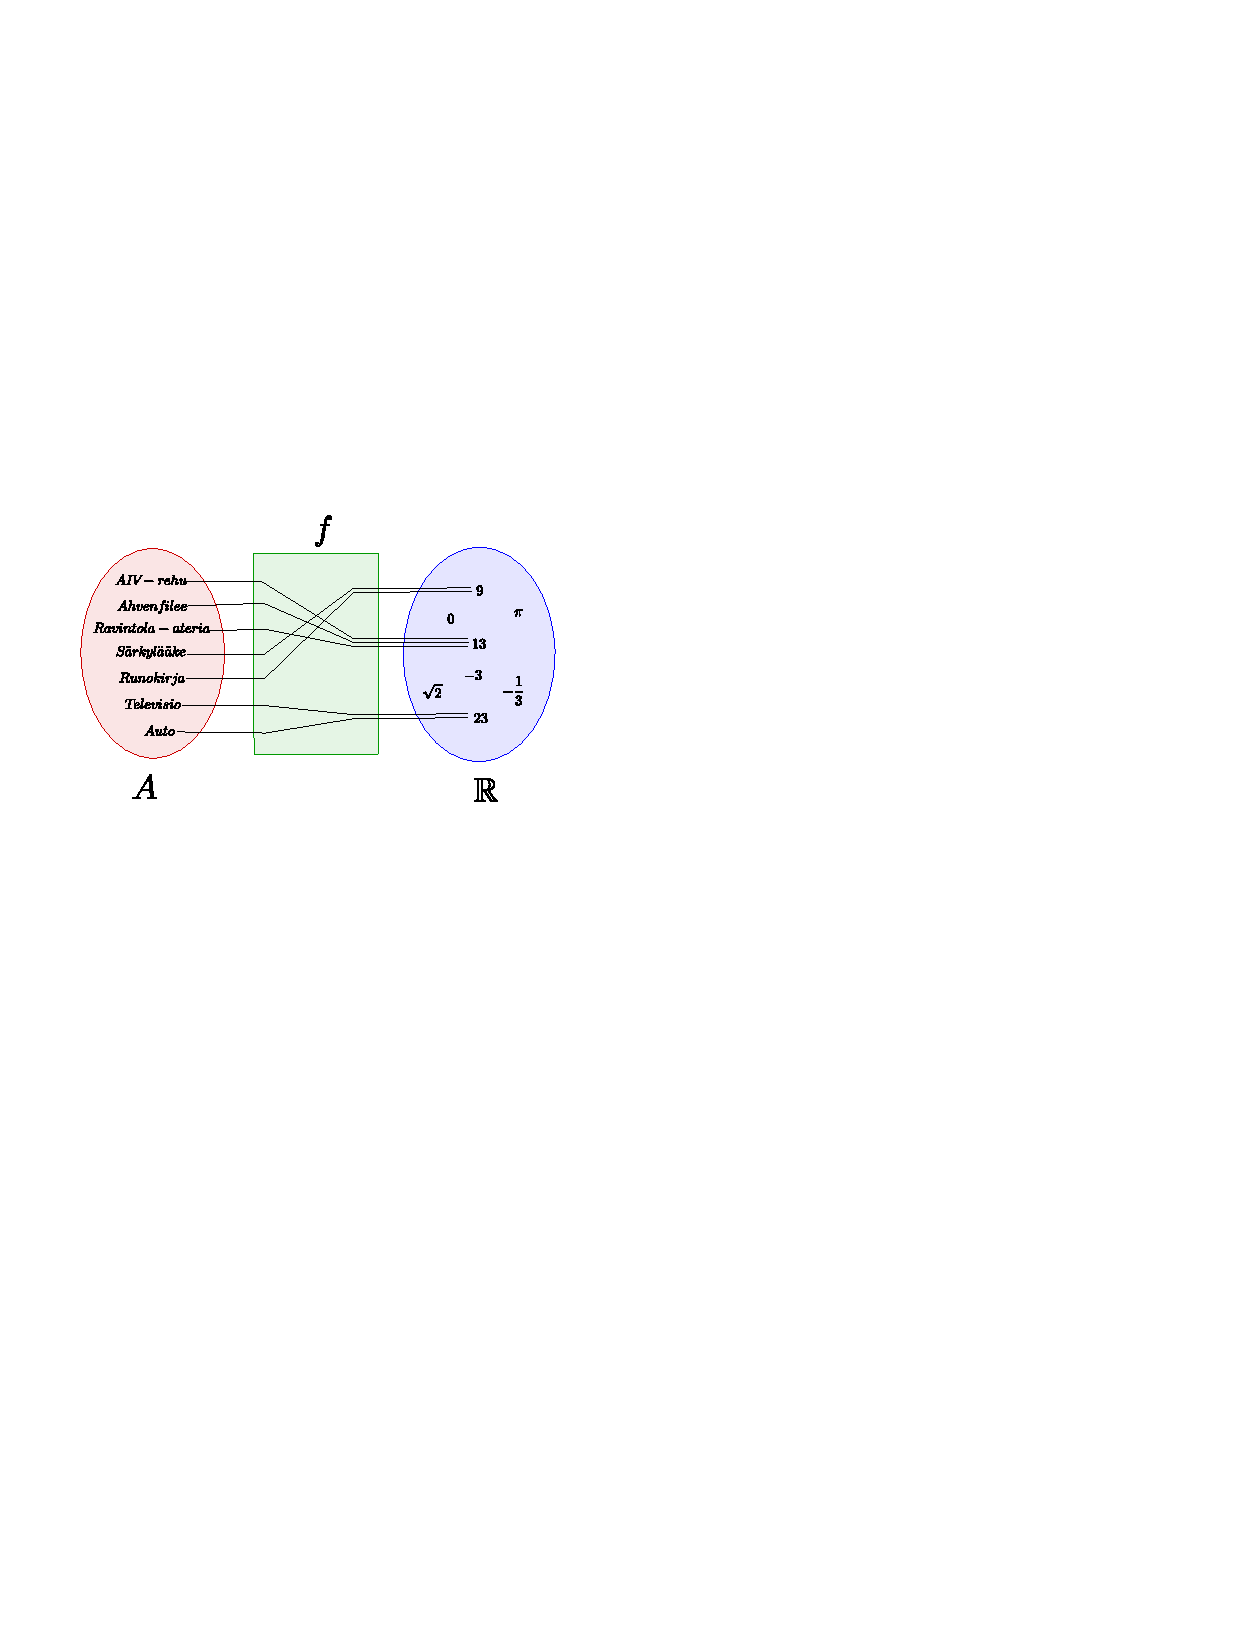
\includegraphics[width=13cm]{03-funktiot/kuvia/funktiokone.pdf}
\end{center}
\end{esimerkki}

Funktioiden käyttämiseen liittyy joitakin vakiintuneita tapoja:
\begin{itemize}
\item $f(x) = y$ lausutaan: ''Funktio saa arvon $y$ pisteessä $x$'',
\item Funktion määrittely- ja arvojoukko jätetään usein merkitsemättä, jos ne voidaan päätellä asiayhteydestä. Tällä kurssilla arvojoukkona on yleensä reaaliluvut.
\item Toisinaan funktiolle ja funktion kuvaajalle ei tehdä selkeää eroa:
$y = f(x)$ samaistetaan koordinaatistoon piirretyn funktion kuvaajan kanssa.
Periaatteessa funktio ja sen kuvaaja ovat kuitenkin eri asioita.
\end{itemize}

Funktiolla on usein jokin selkeä sääntö, joka voidaan kirjoittaa
matemaattisena lausekkeena.

\begin{esimerkki}
Jos neliön sivun pituutta merkitään $x$:llä, voidaan sivun pituuden
ja neliön pinta-alan välistä yhteyttä kuvata funktiolla
$A(x) = x^2$.
\end{esimerkki}

Funktion määrittelyjoukko koostuu niistä muuttujan arvoista, joilla
funktio on määritelty eli joilla funktion arvo voidaan laskea.

\begin{esimerkki}
Määritellään funktio $f$ lausekkeella
\[
f(x) = \frac{1}{x-1}.
\]
Mikä on funktion määrittelyjoukko?

\textbf{Ratkaisu.}
Funktio $f(x)$ on määritelty, kun nimittäjä $x-1$ on erisuuri
kuin 0. Tämä toteutuu kaikilla $x$:n arvoilla lukuun ottamatta
arvoa $x = 1$. Funktion määrittelyjoukkoon kuuluvat siis
kaikki reaaliluvut paitsi luku 1.
\end{esimerkki}

Funktion \emph{arvojoukko} sisältää ne maalijoukon alkiot,
jotka funktio saa arvokseen ainakin yhdessä pisteessä.

\esimerkki{
Mikä on edellä määritellyn funktion $f(x)$ arvojoukko?

\textbf{Ratkaisu.}
Arvojoukon selvittämiseksi tutkitaan, millä luvun $a$ arvoilla
yhtälöllä $f(x) = a$ on ratkaisu,
\begin{align*}
a &= \frac{1}{x-1} & &| \, \text{Oletetaan, että $x \neq 1$, jolloin voimme kertoa $(x-1)$:llä puolittain.} \\
a(x-1) &= 1 \\
x-1 &= \frac{1}{a} \\
x &= 1+\frac{1}{a} & &| \, \text{Havaitaan, että yhtälöllä on ratkaisu
kaikilla $a \neq 0$.}
\end{align*}
Funktion arvojoukko on siis koko reaalilukujen joukko.
}
